\chapter{\IfLanguageName{dutch}{Stand van zaken}{State of the art}}%
\label{ch:stand-van-zaken}

% Tip: Begin elk hoofdstuk met een paragraaf inleiding die beschrijft hoe
% dit hoofdstuk past binnen het geheel van de bachelorproef. Geef in het
% bijzonder aan wat de link is met het vorige en volgende hoofdstuk.

% Pas na deze inleidende paragraaf komt de eerste sectiehoofding.

\section{\IfLanguageName{dutch}{Introductie}{Introductie}}

Het doel van dit hoofdstuk is het onderzoeken en analyseren van bestaande informatie in de vorm van academische literatuur, artikelen en boeken om een duidelijker beeld te krijgen van ons onderwerp. Het onderzoek zal beginnen met het definiëren van het Internet of Things (IoT) en hun communicatieprotocollen. Vervolgens wordt geanalyseerd hoe netwerk gebaseerde intrusiedetectiesystemen (NIDS) ingezet kunnen worden om deze toestellen te monitoren.
\vspace{1em}

Deze tools bieden IT-experts namelijk een gedetailleerd inzicht in netwerkactiviteit, waardoor ze verdacht gedrag kunnen detecteren en volgen.
\vspace{1em}

Ten slot wordt er onderzocht welke uitdagingen kunnen optreden wanneer deze systemen worden gedraaid op Single-Board Computers, zoals de Raspberry Pi.
\vspace{1em}

De kern van dit onderzoek richt zich op het evalueren en vergelijken van het resourcegebruik (CPU- en geheugenbelasting) van open-source detectiesystemen en het bepalen van hun operationele geschiktheid op computerbeperkte hardware binnen een IoT-omgeving voor een klein bedrijf.
\vspace{8em}


\section{\IfLanguageName{dutch}{Internet of Things}{Internet of Things}}

Het internet is geëvolueerd op manieren die we ons niet hadden kunnen voorstellen. Deze groeiende technologie kan het best worden geïllustreerd door het enorme aantal apparaten dat momenteel is aangesloten op het internet, zoals te zien is in Figuur \ref{fig:Aantal_toestellen}.

\begin{figure}[H]
    \centering
    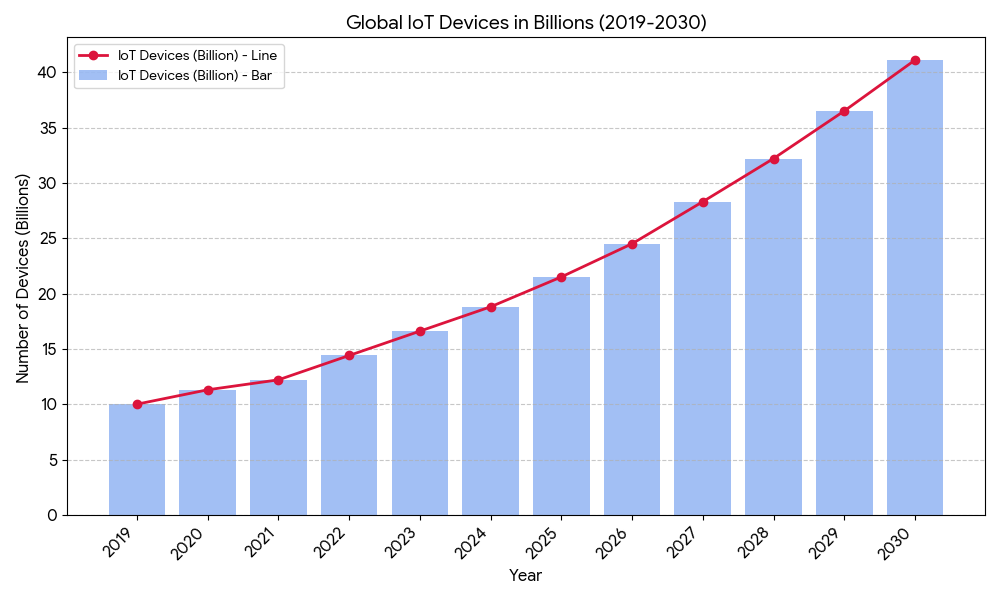
\includegraphics[width=1\textwidth]{../graphics/IoT_groei.png}
    \caption{Voorspelling van de groei van het aantal IoT-toestellen (2019-2030)}
    \label{fig:Aantal_toestellen}
\end{figure}

Volgens data van het platform IoT Analytics, geciteerd in recent onderzoek van \textcite{Sebestyen2025}, zou het aantal aangesloten IoT-apparaten in 2025 jaarlijks met 14\% stijgen tot 21,1 miljard apparaten. Bovendien kunnen we uit de afbeelding afleiden dat dit aantal tegen het jaar 2031 naar verwachting zal zijn verdubbeld.

\vspace{1em}

De term "Internet of Things" (IoT) werd in 1999 voor het eerst geïntroduceerd door Kevin Ashton om een systeem te beschrijven dat radiofrequentie-identificatie (RFID) en andere sensoren gebruikte om de fysieke wereld rechtstreeks met het internet te verbinden \autocite{Lueth2014}.

\vspace{1em}

Na verloop van tijd breidde het concept zich uit tot meer dan alleen het bijhouden van de operationele status.
Vandaag de dag gebruiken wij een gemoderniseerde definitie die opgesteld werd door de International Telecommunication Union (ITU) \autocite{Union2012}:


\begin{center}
    \textit{“A global infrastructure for the information society, enabling advanced services by interconnecting (physical and virtual) things based on existing and evolving interoperable information and communication technologies."}
\end{center}

In tegenstelling tot het oorspronkelijke concept wordt het IoT hier gedefinieerd als een enorm netwerk van fysieke objecten die via het internet communiceren om gegevens te verzamelen, uit te wisselen en te verwerken zonder dat hierbij menselijke interactie vereist is \autocite{Union2012}.

Om te begrijpen hoe deze apparaten binnen een netwerkinfrastructuur met elkaar samenwerken, kan het drielagenmodel \autocite{ijca2021921311} als conceptuele basis  worden gebruikt om de IoT-architectuur te visualiseren Figuur \ref{fig:drie_lagen_model }.
Dit model verdeelt de informatiestroom in drie lagen, namelijk:
\begin{enumerate}
    \item Perceptielaag: Is de fysieke laag die sensoren bevat om gegevens te verzamelen.
    \item Netwerklaag: Verantwoordelijk voor de verbinding met andere apparaten of servers. Omvat ook het verzenden en verwerken van gegevens van sensoren.
	\item Applicatielaag: Verantwoordelijk voor het leveren van applicatieservices aan de gebruikers via gebruikersinterfaces.
\end{enumerate}


\begin{figure}[H]
    \centering
    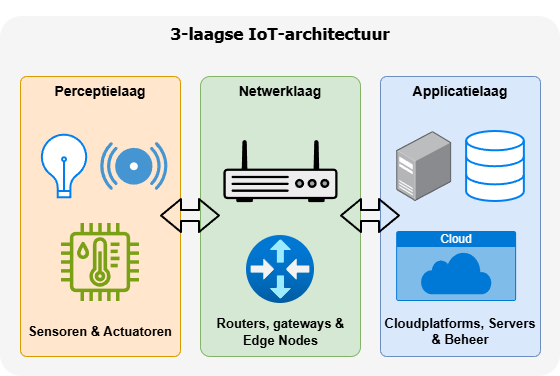
\includegraphics[width=1\textwidth]{../graphics/3-lagenmodel.png }
    \caption{3 Lagen model (IoT-Architectuur)}
    \label{fig:drie_lagen_model }
\end{figure}

\vspace{8em}

\subsection{Communicatieprotocollen}

Het idee van het Internet of Things is in essentie een Machine-to-Machine (M2M) interactie, waarbij apparaten communiceren via een breed scala aan protocollen verspreid over de verschillende lagen van het OSI-model (Figuur: \ref{fig:Osi_model}). 

\vspace{1em}
Omdat IoT-toestellen vaak beperkt zijn in hun hardwarebronnen en rekenkracht, is het gekozen communicatieprotocol gelinkt aan de use case van elk toestel \autocite{s20133637}.
Om een antwoord te kunnen formuleren op de centrale onderzoeksvraag, is de scope van deze literatuurstudie afgebakend tot communicatieprotocollen die direct of indirect zichtbaar zijn voor een Network Intrusion Detection System (NIDS).

\vspace{1em}

Dit betekent IP-gebaseerde protocollen op de hogere lagen van de netwerkstack, zoals MQTT en CoAP. Maar ook draadloze standaarden zoals Zigbee. 

\begin{figure}[H]
    \centering
    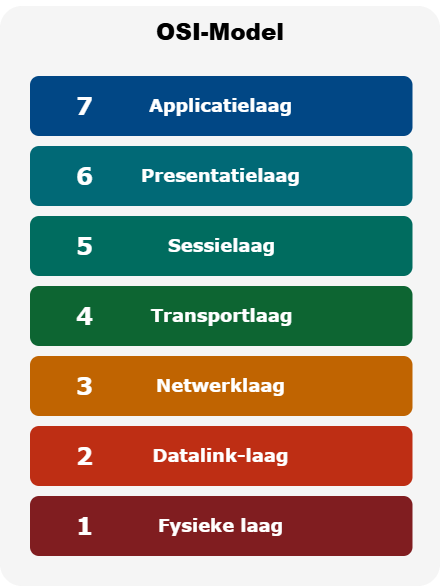
\includegraphics[width=0.4\textwidth]{../graphics/Osi-model.png}
    \caption{Het OSI-model}
    \label{fig:Osi_model}
\end{figure}


Tabel~\ref{tab:iot_protocollen} geeft een overzicht van de meest gebruikte communicatieprotocollen binnen IoT- en webtoepassingen.

\begin{table}[H]
\centering
\small
\renewcommand{\arraystretch}{1.1} % Houdt de rijen verticaal strak en compact
\setlength{\tabcolsep}{8pt}       % Optimale horizontale afstand tussen kolommen
\caption{Vergelijkend overzicht van geselecteerde IoT-communicatieprotocollen en hun NIDS-zichtbaarheid.}
\label{tab:iot_protocollen}
\begin{tabular}{llll}
\toprule
\textbf{Protocol} & \textbf{Transport / Standaard} & \textbf{Communicatiemodel} & \textbf{NIDS-Zichtbaarheid} \\
\midrule
\textbf{MQTT}      & TCP (1883 / 8883) & Publish / Subscribe    & Direct (IP-gebaseerd) \\
\textbf{CoAP}      & UDP (5683 / 5684) & Request / Response     & Direct (IP-gebaseerd) \\
\textbf{HTTP/REST} & TCP (80 / 443)    & Request / Response     & Direct (IP-gebaseerd) \\
\textbf{Zigbee}    & IEEE 802.15.4     & Master / Slave \& Mesh & Indirect (via gateway-vertaling) \\
\bottomrule
\end{tabular}
\end{table}

\subsubsection{Message Queuing Telemetry Transport Protocol (MQTT)}

MQTT is een van de oudste M2M-communicatieprotocollen, geïntroduceerd in 1999 door Andy Stanford-Clark en Arlen Nipper \autocite{Naik2017}. 

Het is een lichtgewicht messaging protocol dat is uitgegroeid tot een van de meest gebruikte communicatiestandaarden in IoT-apparaten. Dit is voornamelijk omdat het specifiek is ontwikkeld voor resource-beperkte apparaten die gericht zijn op lage kosten, open source, betrouwbaarheid en eenvoudige communicatie \autocite{Bay_lm__2022}.

Het protocol werkt volgens een publish/subscribe-architectuur (zie Figuur \ref{fig:MQQT_protocol}). In dit model publiceert de MQTT-client berichten naar een MQTT-broker (die lokaal of in de cloud draait), waarop andere clients zich kunnen inschrijven en waar berichten worden bewaard voor latere aflevering. MQTT gebruikt TCP als standaard transportprotocol en is afhankelijk van \textit{TLS/SSL} voor encryptie.

\begin{figure}[H]
	\centering
	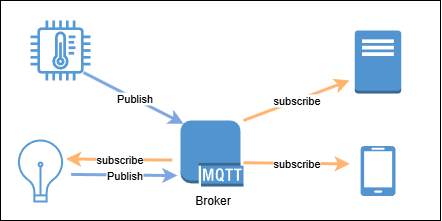
\includegraphics[width=0.7\textwidth]{../graphics/mqttbroker.png}
	\caption{De publish/subscribe-architectuur van MQTT, met de rol van de Broker als centrale communicatiehub.}
	\label{fig:MQQT_protocol}
\end{figure}

\paragraph{MQTT-architectuur: Lokale vs Cloud-brokers}
De groei van MQTT is duidelijk zichtbaar door de adoptie van het protocol door cloudplatforms, waaronder AWS IoT Core (\cite{aws_iot_core})  en Azure IoT Hub (\cite{azure_iot_hub}).

Hoewel dergelijke cloudoplossingen geschikt zijn voor grootschalige IoT-implementaties, maken KMO's vaak gebruik van lokaal gehoste MQTT-brokers (zoals Eclipse Mosquitto) . Deze keuze wordt meestal gedreven door factoren zoals lage operationele kosten en de behoefte aan meer controle over de eigen netwerkinfrastructuur.




\subsubsection{Constrained Application Protocol (CoAP)}

Het CoAP-protocol werd ontwikkeld door de \textit{Constrained RESTful Environment} (CoRe) werkgroep van de IETF \autocite{Bay_lm__2022}. Het is specifiek ontworpen om de REST-architectuur (zie Figuur \ref{fig:REST_arch}) van het reguliere web toe te passen op extreem resource-beperkte apparaten en netwerken met een lage bitrate \autocite{aipcp-2591-030074}.


Omdat de TCP-handshake te veel overhead met zich meebrengt voor kleine sensoren, draait CoAP op de UDP-protocol en maakt gebruik van DTLS (Data Transport Layer Security) voor encryptie \autocite{iot-2020-100264}. Door zijn effectieve en lage overhead is het bezig een standardprotocol te worden voor veel IoT-oplossingen \autocite{Thantharate_2019}.



\subsubsection{HyperText Transport Protocol (HTTP/REST)}

Het HTTP/REST-protocol is het traditionele basisprotocol van het World Wide Web (WWW) dat gebruikmaakt van het TCP-protocol in de transportlaag \autocite{iot-2020-100264}. Hoewel dit protocol perfect is voor standaard client-servercommunicatie (zie Figuur \ref{fig:REST_arch}), is het te zwaar en bevat te veel overhead voor IoT-toestellen \autocite{iciss-2020-9316031}.


HTTP maakt gebruik van tekstgebaseerde headers die vaak honderden bytes kunnen zijn en dit zorgt ervoor dat apparaten met beperkte hardware bronnen de data intensiever moeten processen \autocite{iciss-2020-9316031}. Daarom wordt HTTP binnen een IoT-omgeving vaak ingezet aan de zware kant van een netwerk, zoals bij servers of gateways \autocite{Naik2017}.


\begin{figure}[H]
	\centering
	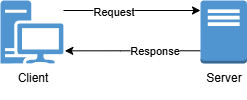
\includegraphics[width=0.4\textwidth]{../graphics/HTTP-ReqRes.png}
	\caption{De request/response-architectuur.}
	\label{fig:REST_arch}
\end{figure}



\subsubsection{Zigbee}

Zigbee werd ontwikkeld door de Connectivity Standards Alliance (CSA) \autocite{iot-2020-100306} als een draadloze standaard met een zeer laag energieverbruik en lage productiekosten voor sensornetwerken.
In tegenstelling tot de eerder besproken protocollen die uitsluitend op de applicatielaag werken, is Zigbee een draadloze mesh-standaard die gebouwd is op IEEE 802.15.4 voor de fysieke en datalinklaag. Het is specifiek ontworpen voor apparaten met een laag energieverbruik en een beperkte rekenkracht \autocite{iot-2020-100306}.

\vspace{1em}

De Zigbee-architectuur is opgebouwd uit drie apparaatrollen:
\begin{enumerate}
    \item \textbf{Zigbee Coordinator (ZC):} De belangrijkste unit die verantwoordelijk is voor het opstarten en configureren van het netwerk, het beheren van de beveiligingssleutels en het opslaan van netwerkinformatie.
    \item \textbf{Zigbee Router (ZR):} Een intermediaire node die gegevens doorstuurt en als repeater werkt om het bereik van het mesh-netwerk te vergroten.
    \item \textbf{Zigbee End Device (ZED):} Dit apparaat bevat enkel de minimale functionaliteit om met een router of de coördinator te communiceren. Het kan gedurende lange perioden in een diepe slaapstand gaan en ontwaakt alleen om sensorwaarden door te geven.
\end{enumerate}

\vspace{1em}

Omdat Zigbee toestellen via een specifieke radiofrequentie op de 2,4 GHz-frequentieband werken, opereren ze buiten de traditionele TCP/IP-stack en is hun verkeer onzichtbaar voor een NIDS. Voor netwerkinspectie en beveiliging moet het verkeer op IP-niveau zichtbaar worden gemaakt via een coördinator en een gateway zoals Zigbee2MQTT.


\section{IDS Security}

Het Intrusion Detection System (IDS) is een beveiligingsoplossing die wordt geïntegreerd in moderne infrastructuren voor het monitoren van netwerkverkeer op verdachte activiteiten of beleidsschendingen. Het primaire doel van een IDS is het identificeren van een potentiële beveiligingsincidenten en dit aan een beheerder waarschuwen, zoals ongeautoriseerde toegangspogingen, malware-infectie of verdachte netwerkverkeerpatronen \autocite{LIAO201316}.

\vspace{1em}

Een IDS wordt vaak beschouwd als een extra security laag die regelmatig wordt gekoppeld met een Intrusion Prevention System (IPS) om dreigingen actief te blokkeren \autocite{inproceedings}. Het IDS focust alleen op het genereren van een alert en de systeembeheerder te informeren van het incident. Deze alerts bevatten informatie over het incident, zoals welke computer of welk netwerksegment is getroffen, evenals aanvullende details die ondersteuning bieden bij de respons en het herstelproces.

\vspace{1em}
Er zijn drie verschillende detectietypen voor IDS en deze kunnen worden ingedeeld in drie categorieën:

\begin{enumerate}
    \item \textbf{Host-gebaseerd IDS (HIDS):} Bewaakt één specifiek systeem. In de meeste gevallen draait de IDS-software direct op de host zelf. Het analyseert systeemlogs en lokale activiteiten om afwijkingen of ongeautoriseerde wijzigingen te detecteren.
    
    \item \textbf{Netwerkgebaseerd IDS (NIDS):} Bewaakt een volledig netwerksegment. Het systeem inspecteert al het binnenkomende en uitgaande verkeer dat een specifiek punt in het netwerk passeert. Hierbij luistert de netwerkinterfacekaart (vaak in \textit{promiscuous mode}) naar alle datapakketten voor analyse.
    
    \item \textbf{Hybride IDS:} Een gecombineerde aanpak waarbij zowel host-gebaseerde als netwerkgebaseerde IDS-sensoren gelijktijdig worden ingezet. Dit biedt een integraal beveiligingsbeeld van zowel het netwerkverkeer als de individuele systemen.
\end{enumerate}

\vspace{1em}
Terwijl een IDS op verschillende locaties kan worden ingezet, kan ook het detectiemodel verschillen. Er zijn voornamelijk twee methodologieën die een IDS gebruikt om een bedreiging te identificeren.

\begin{enumerate}
    \item \textbf{Handtekening-gebaseerde detectie (Signature-based):} Dit model maakt gebruik van een database met bekende aanvalspatronen of "handtekeningen". Het IDS vergelijkt de actuele netwerkactiviteiten met deze database; zodra er een overeenkomst wordt gevonden met een herkende aanval, genereert het systeem direct een waarschuwing.
    
    \item \textbf{Anomalie-gebaseerde detectie (Anomaly-based):} In dit model definieert het IDS een "normale toestand" (baseline) van het netwerk of de specifieke host. Het systeem leert hoe legitiem gebruikersgedrag eruitziet. Wanneer er een afwijking van deze basislijn optreedt, wordt dit gerapporteerd als een potentiële aanval. Een nadeel van dit model is dat het kan leiden tot een hoger aantal vals-positief meldingen (false positives) \autocite{Patcha2007Anomaly}.
\end{enumerate}


\paragraph{Scope van het onderzoek}
In de context van het IoT is de implementatie van HIDS op eindapparaten niet haalbaar vanwege de minimale rekenkracht en het ontbreken van een volwaardig besturingssysteem. Om deze reden richt dit onderzoek zich voornamelijk op het controleren en inspecteren van netwerkverkeer op gateway- of switch-niveau. Door een IDS op het netwerkniveau te implementeren, kunnen afwijkingen en anomalieën detecteren zonder de aangesloten IoT-apparaten zelf te belasten.


\subsection{Suricata: Handtekening-gebaseerde detectie}

Suricata is een krachtige, open-source engine voor het detecteren en voorkomen van bedreigingen, ontwikkeld door de Open Information Security Foundation (OISF) \autocite{SuricataDocs2024}. Deze netwerkmonitoringtool is geschikt voor het uitvoeren van Network Intrusion Detection (NIDS), Network Intrusion Prevention (NIPS) en passieve Network Security Monitoring (NSM) \autocite{Amoretti2025}.

Het detectiemodel dat Suricata gebruikt, is een \textbf{\textit{Handtekening-gebaseerde detectie}} model, waarbij het netwerkverkeer op meerdere lagen wordt onderzocht en vergeleken met opgeslagen signaturen of regels \autocite{SuricataFeatures2024}.

Omdat Suricata Snort-compatibele regelformaten en syntaxis ondersteunt, bestaan er community regelsets (zoals de ETOpen) die snel geïmplementeerd kunnen worden \autocite{SuricataRulesDiff2024}.




\subsection{Zeek: Anomalie-gebaseerde detectie}

Zeek, ook bekend als Bro \autocite{icaccs-2022-9785047}, is een passieve, opensource netwerkverkeersanalyser die veel gebruikt wordt als een Network Security Monitor (NSM) tool, gericht op diepe netwerkanalyse \autocite{ZeekDocs}. 
 
In tegenstelling tot traditionele, op handtekening-gebaseerde detectiemodellen zoals Suricata, analyseert Zeek netwerkpakketten en structureert het deze in een zeer overzichtelijke logboekdatabase. De gegenereerde logs kunnen variëren afhankelijk van het type verkeer dat door Zeek stroomt, waarbij de data per protocol in afzonderlijke logbestanden wordt opgesplitst (Figuur: \ref{fig:ZeekLog}).

\begin{figure}[H]
    \centering
    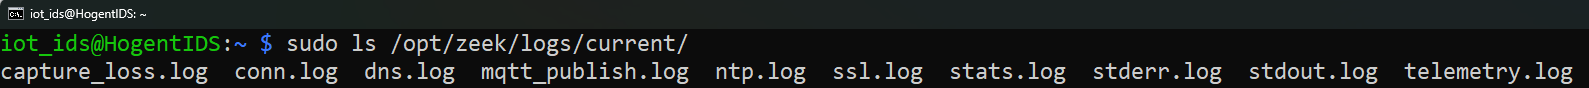
\includegraphics[width=1\textwidth]{../graphics/ZeekLog.png}
    \caption{Overzicht van de protocol-specifieke telemetriebestanden binnen de actieve Zeek log-directory (/opt/zeek/logs/current/). }
    \label{fig:ZeekLog}
\end{figure}


Bovendien beschikt Zeek over een eigen, complete scripttaal \autocite{ZeekDocs} waarmee systeembeheerders aangepaste netwerklogica kunnen programmeren. In plaats van gebonden te zijn aan statische regelsets, maakt Zeek gebruik van deze scripts voor potentiële aanvallen op te sporen en melden.
